%%%%%%%%%%%%%%%%%%%%%%%%%%%%%%%%%%%%%%%%%%%%%%%%%%%%%%%%%%%%%%%%%%%%%%%%%%%%%%%%%%%%%%%%%
%%%%%%%%%%%%%%%%%%%%%%%%%%%%         MANUFACTURING PLAN        %%%%%%%%%%%%%%%%%%%%%%%%%%
%%%%%%%%%%%%%%%%%%%%%%%%%%%%%%%%%%%%%%%%%%%%%%%%%%%%%%%%%%%%%%%%%%%%%%%%%%%%%%%%%%%%%%%%%

 \section{Manufacturing Plan} % (15 Points)
\label{sec:ManufacturingPlan}
% Section Requirements:
% 1) Preliminary manufacturing flow
% 2) Describe critical processes or technologies required


%%%%%%%%%%%%%%%%%%%%%%%%%%%%%%%%
%%%% - Manufacturing Flow - %%%%
%%%%%%%%%%%%%%%%%%%%%%%%%%%%%%%%
\subsection{Manufacturing Flow}
\label{ssec:ManufacturingFlow}

%Manufacturing flow figure. Move around to get formatting right.
\begin{wrapfigure}[9]{R}{0pt}
	\centering
	\raisebox{0pt}[\dimexpr\height-3\baselineskip\relax]{ %NOTW: CHANGE THIS - VALUE TO SHIFT THE FIGURE UP INTO THE SECTION TITLE AREA IF YOU NEED TO.  OTHERWISE, COMMENT OUT THIS LINE
		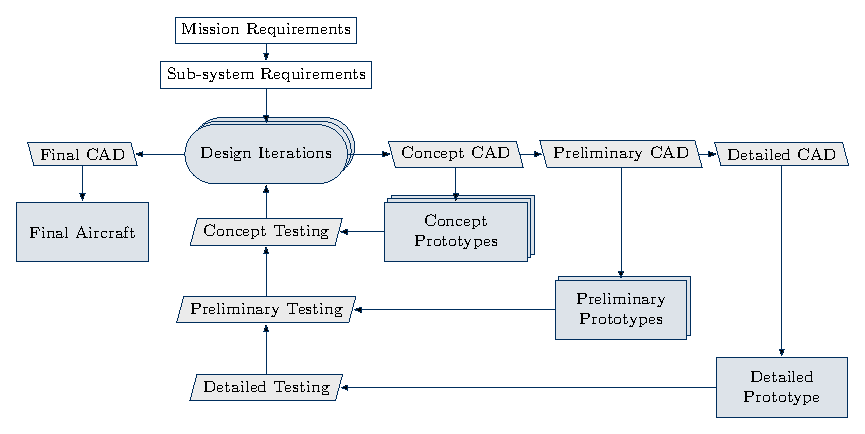
\includegraphics[width=0.6\textwidth]{manufacturing_flow}
	} %NOTE: IFF YOU COMMENT OUT THE \RAISEBOX LINE ABOVE, COMMENT OUT THIS LINE TOO.
	\caption{Our 3-phase design, build, fly plan enables a more robust final aircraft.}
	\label{fig:manufacturingplan}
\end{wrapfigure}

Our manufacturing flow follows the outline found in \cref{fig:plannedtiming} which includes three design-build-fly phases.  \Cref{fig:manufacturingplan} shows this flow with more clarity.  Note that for all phases, CAD will commence roughly a week after design starts, prototyping a week after that.

\subsubsection{Phase 1} We began with a conceptual design along with conceptual CAD, from which we have built concept prototypes to be used in testing as described below. {\color{BYUred}[ADD A DETAIL ABOUT MATERIALS AND/OR PROCESSES.]}

\subsubsection{Phase 2} We are currently beginning our preliminary design and CAD from which we will build preliminary prototypes for testing. {\color{BYUred}[ADD A DETAIL ABOUT MATERIALS AND/OR PROCESSES.]}

\subsubsection{Phase 3} Around the new year, we will start on our detailed design and CAD, which will lead to our final testing prototypes.  After polishing the design and CAD after final testing, we will manufacture our final competition aircraft. {\color{BYUred}[ADD A DETAIL ABOUT MATERIALS AND/OR PROCESSES.]}



%%%%%%%%%%%%%%%%%%%%%%%%%%%%%%%%
%%%% - Critical Processes - %%%%
%%%%%%%%%%%%%%%%%%%%%%%%%%%%%%%%
\subsection{Critical Processes}
\label{ssec:CriticalProcesses}

{\color{BYUred}[YOU NEED TO DISCUSS THE CRITICAL PROCESSES AND TECHNOLOGY BASED ON HOW YOU'VE DECIDED TO MANUFACTURE THINGS THIS YEAR.  FOAM CUTTING? 3D PRINTING? LASER CUTTING? ETC.]}
\lipsum[3]

